\section{Reconocimiento de texto}
	\begin{frame}
		\begin{center}
			\begin{huge}
				{Reconocimiento de texto}
			\end{huge}
		\end{center}
	\end{frame}
	\subsection{Concepto}
		\begin{frame}
			\frametitle{Reconocimiento de texto}
			El reconocimiento de texto es el proceso por el cual, dada una imagen, se identifican las zonas que contienen texto y se extrae la información de estas con el objetivo de poder digitalizarlas para su posterior procesamiento, análisis o almacenamiento, entre otros.
		\end{frame}
		\begin{frame}
			\frametitle{OCR}		
			\textit{OCR} o \textit{Reconocimiento óptico de caracteres} es una de las etapas del reconocimiento de texto. Es un proceso que tiene como objetivo identificar símbolos o caracteres que pertenecen a un determinado alfabeto.
		\end{frame}
	\subsection{Comienzos}
		\begin{frame}
			\frametitle{OCR: comienzos}
			\begin{itemize}
				\item<1-> Objetivo: \textit{Documentos escaneados}
				\item<2-> Se realizaba con máquinas.
				\item<3-> Se registran sus inicios en 1914 cuando Edmund Fournier desarrolla el \textit{Optophone}.
			\end{itemize}
			\begin{center}
				\includegraphics<3>[height=0.45\paperheight]{../img/Optophone.jpg}
			\end{center}
		\end{frame}
	\subsection{Actualidad}
		\begin{frame}
			\frametitle{OCR: actualidad}
			\begin{itemize}
				\item<1-> Objetivo: todo lo que contenga texto. Desde \textit{documentos escaneados} hasta \textit{imágenes naturales}.
				\item<2-> Se realiza principalmente a través de software.
			\end{itemize}
		\end{frame}
	\subsection{Pipeline}
		\begin{frame}
			\frametitle{Pipeline de procesamiento: Documento escaneado}
			\begin{center}
				\includegraphics<1>[height=0.65\paperheight]{imgs/texto_plano.png}
				\includegraphics<2>[height=0.65\paperheight]{imgs/texto_plano_det_texto.png}
				\includegraphics<3>[height=0.65\paperheight]{imgs/texto_plano_det_palabras.png}	
				\includegraphics<4>[height=0.65\paperheight]{imgs/texto_plano_det_caracteres.png}
			\end{center}
		\end{frame}
	\subsection{Imagenes naturales}
		\begin{frame}
			\frametitle{Problema: Imágenes naturales}
			\begin{center}
				\includegraphics<1>[height=0.65\paperheight]{imgs/imagen_natural_1.jpg}
				\includegraphics<2>[height=0.65\paperheight]{imgs/imagen_natural_2.jpg}
				\includegraphics<3>[height=0.65\paperheight]{imgs/imagen_natural_3.jpg}
				\includegraphics<4>[height=0.65\paperheight]{imgs/imagen_natural_4.jpg}	
			\end{center}
		\end{frame}
		\begin{frame}
			\frametitle{Caracteres en imágenes naturales}
			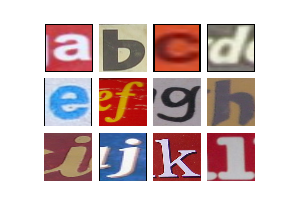
\includegraphics[height=0.65\paperheight]{imgs/caracteres_naturales.png}	
		\end{frame}
		\begin{frame}
			Texto escaneado:
			\begin{itemize}
				\item Fondo es homogeneo.
				\item No hay tanto ruido como en las imágenes naturales.
				\item Los palabras se muestran de frente y alineadas.
				\item Los caracteres tienen la misma forma y tamaño.
			\end{itemize}
		\end{frame}
		\begin{frame}
			Imagen natural:
			\begin{itemize}
				\item Fondo complejo.
				\item Presencia de elementos que dificultan la tarea de reconocimiento:
				\begin{itemize}
					\item Iluminación
					\item Ruido Gaussiano o Blur.
					\item Oclusión
					\item Etc.
				\end{itemize}
				\item Las palabras pueden estar dispuestas en diferentes ángulos y perspectivas (depende de la posición al momento de tomar la foto).
			\end{itemize}
		\end{frame}
